%%%%%%%%%%%%%%%%%%%%
%
% $Autor: Wings $
% $Datum: 2020-02-24 14:29:03Z $
% $Pfad: komponenten/Bilderkennung/Produktspezifikation/CorelTPU/Ausarbeitung/Kapitel/Software.tex $
% $Version: 1791 $
%
%
%%%%%%%%%%%%%%%%%%%


%todo \url{https://www.kdnuggets.com/2017/09/tensorflow-tutorial-part-1.html}
%todo \url{https://www.kdnuggets.com/2017/09/tensorflow-tutorial-part-2.html}


    
\chapter{TensorFlow} \label{Kapitel_TF}

\section{TensorFlow 2.0} 
 
 TensorFLow ist eine Open Source-Bibliothek für Deep Leanring, auf Grund ihres Umfangs häufig auch als Framework bezeichnet.
Seit 2019 steht die freie Bibliothek in der Verson 2.0 zur Verfügung. Der Umfang der Bibliothek hat dazu geführt, 
dass sie sowohl in der Wissenschaft als auch in der Industrie vielfach eingesetzt wird. Die aktuelle Version 2.0 wurde am 30. September 2019 veröffentlicht.
 \cite{TensorFlow.02.12.2020}

Die Open-Source-Bibliothek verwendet Datenflussgraphen zur Erstellung von Modellen. 
Sie ermöglicht es Entwicklern, große neuronale Netze mit vielen Schichten zu erstellen. TensorFlow wird hauptsächlich verwendet für: Klassifikation, Wahrnehmung, Verstehen, Entdecken und Vorhersagen. \cite{GoogleTensorFlow:2019} %Quelle prüfen

\section{TensorFlow und Python}
Laut \cite{Heise:2020} ist das Python-API bei TensorFlow und Co. die vollständigste und verbreitetste Schnittstelle. Daher ist es sinnvoll, sich mit Python vertraut zu machen, wenn man mit TensorFlow arbeiten möchte.
Für Python spricht zum einen die übersichtliche Struktur mit Einrückungen zur Abgrenzung von Blöcken. Das macht den Code kompakt und gut lesbar. Gleichzeitig ist Python vielseitig einsetzbar, vom Bash-Skript-Ersatz bis zum neuronalen Netz. Besonders experimentieren und herumprobieren ist mit Python einfach und schnell möglich, da Python den Code direkt ohne Kompilieren in Maschinencode interpretiert. Zudem können viele hilfreiche libaries importiert und verwendet werden.
Als Nachteil gilt jedoch die Rechenzeit in Python. Dennoch gilt es als die Sprache der KI-Forschung. Dieser Widerspruch erklärt sich so, dass Frameworks wie Caffe oder TensorFlow genutzt werden, die \glqq ihre Berechnungen automatisch für
die vorhandene Hardware optimieren und dabei
beispielsweise den CUDA-Compiler anwerfen, um
auf der Grafikkarte zu rechnen.\grqq \cite{Heise:2020}

Häufig wird Python innerhalb von Jupyter Notebook verwendet. Die Notebooks erlauben das sequentielle Ausführen einzelner Code-Blöcke und Visualisierungen und lassen sich im Browser öffnen und bearbeiten. Dafür muss neben Jupyter Notebook auch eine aktuelle Version von Python auf dem PC installiert sein. Empfohlen wird der Download der Anaconda-Distribution, die Jupyter Notebook und Python zusammen mit weiteren nützlichen Software-Paketen für Datenwissenschaft und Co. installiert. Anschließend kann über das Anaconda Prompt mit der Eingabe 'Jupiter Notebook' selbiges im Browser geöffnet werden.


\section{Installation von TensorFlow}

Neben der Standardversion der Bibliothek existieren auch Varianten, die
spezielle Hardware unterstützen. Neben der Standardvariante werden hier auch
Variante für Intel-Hardware und für NVIDIA-Grafikkarten vorgestellt.


\subsection{Standard}

%todo

Installation der Bibliothek erfolgt bei einer Anaconda-Installation wie folgt:

Zuerst muss das Anaconda Prompt geöffnet werden. Dann sollte zuerst mit

\medskip 
\SHELL{\$ pip install --upgrade pip}
\medskip

die aktuellste Version von pip installiert werden. 

Dabei kann eine Fehlermeldung bezügliche verweigerten Zugriffs auftreten, die empfiehlt, den Befehl entsprechend anzupassen:

\medskip
\SHELL{\$ pip install --upgrade pip --user}
\medskip

Die durch das zuvor fehlgeschlagene Upgrade geschädigte pip-Version kann repariert werden mit

\medskip
\SHELL{\$ easy\_install pip}
\medskip

Die Installation von TensorFlow erfolgt schließlich mit

\medskip

\SHELL{\$ pip install tensorflow}


\subsection{Installation für Intel-Hardware} %korrekt?

Intel hat für seine Hardware, wie zum Beispiel der Intel Neural Compute Stick 2, die Bibliothek 
optimiert. Die Installation von TensorFlow erfolgt speziell 
für Intel-Hardware beispielsweise durch folgende Kommandos:

\medskip

\SHELL{\$ conda install –c intel tensorflow}


\medskip


\subsection{Installation für Jetson Nano}
Auf der NVIDIA-Seite wird die Installation von TensorFlow für NVIDIA, in diesem Fall für den Jetson nano beschrieben.\cite{NVIDIA.27.10.2020}

System packages installieren, die von TensorFlow benötigt werden:

\SHELL{\$ sudo apt-get update}
\SHELL{\$ sudo apt-get install libhdf5-serial-dev hdf5-tools libhdf5-dev zlib1g-dev zip libjpeg8-dev liblapack-dev libblas-dev gfortran}
\medskip

Pip3 installieren und aktualisieren:

\SHELL{\$ sudo apt-get install python3-pip}
\SHELL{\$ sudo pip3 install -U pip testresources setuptools==49.6.0} 
\medskip

Python Package Abhängigkeiten installieren:

\SHELL{\$ sudo pip3 install -U numpy==1.16.1 future==0.18.2 mock==3.0.5 h5py==2.10.0 keras\_preprocessing==1.1.1 keras\_applications==1.0.8 gast==0.2.2 futures protobuf pybind11}

\medskip

Das Ausführen des letzten Kommandos kann einige Minuten in Anspruch nehmen. Dies ist normal, auch wenn zwischenzeitlich
kein Forstschritt der Aktivität ersichtlich ist.

\medskip

Installieren einer zur JetPack-Version passenden TensorFlow-Version:
\SHELL{\$ sudo pip3 install --extra-index-url https://developer.download.nvidia.com/compute/redist/jp/v\$JP\_VERSION tensorflow}
\medskip

Für <\$JP\_VERSION> muss die installierte JetPack-Version eingesetzt werden, wobei 44 für die Version 4.4 und 45 für 4.5 steht usw.
Die installierte Version kann durch die Eingabe
\SHELL{dpkg-query --show nvidia-l4t-core}
und Abgleich der L4T-Nummer mit den jeweiligen JetPack-Versionen auf der Seite \url{https://developer.nvidia.com/embedded/jetpack-archive}
bestimmt werden.
Auch das Ausführen dieses Schrittes benötigt einige Minuten.


\section{\glqq Hello World\grqq des Maschinellen Lernens - Handgeschriebene Ziffern}

Das typische erste Programm im Deep Learning ist die Erkennung von handgeschriebenen Ziffern aus dem MNIST-Datensatz. 
Auch auf der \href{https://www.tensorflow.org/}{TensorFlow-Wepgage} findet sich unter dem 
\href{https://www.tensorflow.org/tutorials/quickstart/beginner}{Schnellstart für Anfänger} 
ein kurzes Tutorial zum Training eines Neuronalen Netzes auf Grundlage des MNIST-Datensatzes. 
Da dieses jedoch sehr kurz gehalten ist,
soll sich die folgende Anleitung an dem Tutorial aus \cite{Heise:2020} orientieren.

Um das neuronale Netz trainieren zu können, muss die entsprechende Abfolge in der Prozesskette
eingehalten werden.


\begin{enumerate}
  \item Laden und Testen des Datensatzes MNIST als Datensatz, der von TensorFlow zur Verfügung gestellt wird
  \item Normalisierung der Bilder in Gleitkommazahlen
  \item Mischen und Formen einer Trainingsabfolge (batch) mit einer definieren Anzahl an Beispielen
  \item Erstellen des neuronalen Netzes und Optimierung mit \PYTHON{Adam}
  \item Spezifikation einer zusätzlichen metrischen Genauigkeit und 
        Trainieren/Test des Modells durch Aufruf der Funktion \PYTHON{model.fit}
\end{enumerate}

\subsection{MNIST-Datensatz}
Der MNIST-Datensatz ist zum freien Gebrauch verfügbar und enthält 70.000 Bilder von handgeschriebenen Ziffern mit den entsprechenden korrekten Klassifikation. 
Der Name des Datensatzes stammt aus der Tatsache, dass es sich um ein \textbf{m}odifiziertes Subset aus zwei Datensätzen des US 
'\textbf{N}ational \textbf{I}nstitute of \textbf{S}tandards and \textbf{T}echnology' handelt. Diese enthalten handgeschriebene Ziffern 
von 250 verschiedenen Personen (Angestellte des US Census Bureau und High School Schüler). Die so gesammelten Datensätze NIST 
Special Database 3 und Special Database 1 wurden zusammengelegt, da ersteres sauberere und leichter zu erkennende Daten enthält 
(dies sind die Daten der Büroangestellten). Zunächst wurde SD-3 als Trainingsset und SD-1 als Testset verwendet, doch auf Grund der 
Unterschiede ist eine Vermengung beider sinnvoller. Der Datensatz ist bereits in 60.000 Trainingsbilder und 10.000 Testbilder aufgeteit. 
\cite{LeCun:2013} \cite{Nielsen:2015}

Bei den Bildern im MNIST Datensatz handelt es sich um Graustufenbilder der Größe $28 \times 28$ pixel.\cite{LeCun:2013}

Die Daten werden in vier Dateien zur Verfügung gestellt, zwei für den Trainingsdatensatz und zwei für den Testdatensatz, wovon eine Datei die Bilddaten 
und die andere die zugehörigen Labels enthält:


\begin{itemize}
  \item train-images-idx3-ubyte.gz:  training set images (9912422 bytes)
  \item train-labels-idx1-ubyte.gz:  training set labels (28881 bytes)
  \item t10k-images-idx3-ubyte.gz:   test set images (1648877 bytes)
  \item t10k-labels-idx1-ubyte.gz:   test set labels (4542 bytes)
\end{itemize}

Die Daten liegen im IDX Dateiformat vor und können so nicht standardmäßig geöffnet und visualisiert werden. 
Man kann aber ein Programm schreiben um die Daten in das CSV-Format zu überführen oder direkt von anderen in das CSV-Format 
überführte Datensätze herunterladen. \cite{Redmon.04.12.2020}


Die Bibliothek TensorFlow stellt den Datensatz MNIST unter \PYTHON{tensorflow\_datasets} selbst zur Verfügung. Eine Liste aller
Datensätze, die über so geladen werden können, ist unter \url{https://www.tensorflow.org/datasets/catalog/overview#all_datasets}
zu finden.


\begin{figure}
  \GRAPHICSC{0.8}{1.0}{TensorFlow/MNISTDataset2}
  \caption{MNIST-Daten \cite{Siddique:2019}}
\end{figure}


\subsection{Laden des Datensatzes}

Durch den Befehl \PYTHON{load\_data()} werden die Daten, sofort 
in zwei Teile aufgeteilt, geladen. Die Daten enthalten dann je zwei Listen, wobei die erste Liste die Bilder enthält und
die zweite Liste die zugehörige Klassifikation. Die Bilder werden in der Liste mit der Bezeichnung \PYTHON{x} geladen,
die Klassifikation mit \PYTHON{y}.

\medskip

\begin{verbatim}
from tensorflow.keras.datasets import mnist
train_da, test_da = mnist.load_data()
x_train, y_train = train_da
x_test, y_test = test_da
\end{verbatim}


\subsubsection{Normalisierung des Bilder}

Ein neuronales Netz erwartet Daten als 32-Bit-Gleitkommazahlen im Wertebereich von $0$ und $1$.
Im folgenden Code werden die Bilddaten daher entsprechend normalisiert und in das Format $28 \times 28$ 
(abhängig von der Netzarchitektur) gebracht.


\begin{verbatim}
import tensorflow.keras.backend as K
from tensorflow.keras.utils  import to_categorical

dat_form = K.image_data_format()
rows, cols = 28, 28
train_size = x_train.shape[0]
test_size = x_test.shape[0]

if dat_form == 'channels_first':
    x_train = x_train.reshape(train_size, 1, rows, cols)
    x_test = x_test.reshape(test_size, 1, rows, cols)
    input_shape = (1, rows, cols)
else:
    x_train = x_train.reshape(train_size, rows, cols, 1)
    x_test = x_test.reshape(test_size, rows, cols, 1)
    input_shape = (rows, cols, 1)

# norm data to float in range 0..1
x_train = x_train.astype('float32')
x_test = x_test.astype('float32')
x_train /= 255
x_test /= 255

# conv class vecs to one hot vec
y_train = to_categorical(y_train,10)
y_test = to_categorical(y_test, 10)
\end{verbatim}

\subsection{Vorbereituung des Trainings}

Statt mit allen Trainingsdaten loszulegen, werden die Daten zunächst auf 100
Bilder beschränkt um die Trainingszeit für die ersten Versuche zu reduzieren:

\medskip

\begin{verbatim}
x_train = x_train[:100]
y_train = y_train[:100]
\end{verbatim}

Bevor das Modell genutzt werden kann, muss es aufgebaut werden. 
Dazu müssen zuerst die zu nutzenden Module importiert werden. Dieses Modell wird mit der Klasse Sequential erzeugt.
Zunächst wird ein sehr einfaches Modell verwendet, das aus nur zwei Schichten besteht.

\medskip

\begin{verbatim}
from tensorflow.keras.models import Sequential
from tensorflow.keras.layers import Dense,Flatten
model = Sequential()
model.add(Flatten())
model.add(Dense(10,activation='softmax'))
\end{verbatim}

\medskip

Der Befehl \PYTHON{Flatten()} verwandelt die Eingabedaten,
hier ein Feld mit 28 mal 28 Einträgen, in einen eindimensionalen 
Vektor der Größe 784. Die Funktion \PYTHON{model.add()} fügt die
Berechnungen jeweils als eigene Schicht zum Modell hinzu.
Anschließend wird mit dem Befehl \PYTHON{Dense()} die 
Berechnung der Aktivierungsfunktion der Neuronen gestartet. 
In diesem Fall sind es zehn Neuronen und die Aktivierungsfunktion 
\PYTHON{softmax}.
Jedem Neuron wird durch die Funktion \PYTHON{softmax}  eine Wahrscheinlichkeit zugeordnet,
so dass die Summe aller Neuronen 1 ist. Ein Wert nahe 1 ist so zu interpretieren, dass das zugehörige Ergebnis mit hoher Sicherheit
angenommen werden kann. Sind alle Werte nahe 0, kann keine sichere Aussage getroffen werden.


TensorFlow baut anhand der obigen Konstruktion einen Graphen für die Berechnungen 
auf, diese werden automatisch optimiert und in ein Format transformiert, das eine effiziente Berechnung
auf der Hardware erlaubt. Je nach Verfügbarkeit werden
KI-Beschleuniger und Grafikkarten unterstützt.

Im praktischen Einsatz werden die Werte von der Eingabe bis zur Ausgabe berechnet.
Zum Training bestimmt TensorFlow automatisch die Ableitung der
loss-Funktion und fügt die Berechnungen mit dem Gradientenabstieg zum Graphen hinzu.
Dazu genügt eine Funktion:

\begin{verbatim}
from tensorflow.keras.losses import categorical_crossentropy
from tensorflow.keras.optimizers import Adam
model.compile(
loss=categorical_crossentropy,
optimizer=Adam(),
metrics=['accuracy'])
\end{verbatim}

Durch den Befehl wird dem Modell die loss-Funktion \PYTHON{categorical\_crossentropy}
übergeben. Die loss-Funktion berechnet den quadratischen euklidischen Abstand zweier Vektoren.
Zur Bestimmung der optimalen Gewichte im neuronalen Netz wird der Algorithmus \PYTHON{Adam()}
verwendet, der eine  Variante des Gradientenabstiegs ist. Der Algorithmus ist sehr robust, so dass 
für die meisten Anwendungen keine Änderungen der Parameter notwendig sind.
Durch den Übergabeparameter \PYTHON{metrics=['accuracy']} wird während der Berechnungen  
gezählt, wie viele Bilder durch das neuronale Netz korrekt bestimmt worden sind.


\subsection{Training}

Das Training kann mit dem Befehl \PYTHON{model.fit()} gestartet werden:

\begin{verbatim}
history = model.fit(x_train, y_train,
	batch_size=128,
	epochs=12, verbose=1,
	validation_data=(x_test, y_test))
\end{verbatim}

Die Funktion erwartet mehrere Parameter. Zunächst müssen die Trainingsdaten 
übergeben werden, gefolgt von den Klassifizierungen. Der dritte Wert ist die
Batchgröße, sie gibt an wie viele Daten gleichzeitig zur Berechnung hinzugezogen
werden. Einerseits soll der Wert möglichst groß sein, um ein gutes Ergebnis zu erzielen, andererseits
ist der Wert durch die Hardware begrenzt. Denn alle Eingangsdaten eines Batchs werden gleichzeitig im Speicher 
des Rechners verarbeitet. Der Parameter \PYTHON{epochs} gibt an, wie oft die Trainingsdaten eines Batchs
beim Training durchlaufen werden. Für komplexere Probleme werden unter Umständen mehr Epochen und eine kleinere Lernrate 
benötigt.


Nach jedem Trainingsdurchlauf kann mittels dem Befehl \PYTHON{validation\_data=(x\_test, y\_test)}
ermittelt werden, wie gut das Modell bei ihm unbekannten Daten abschneidet.

Der Rückgabewert der Funktion \PYTHON{model.fit()} ist ein Objekt \PYTHON{history}.
Mit Hilfe diese Objekts kann der Lernerfolg verfolgt werden.
Die Visualisierung kann mit TensorBoard erfolgen, wie im nächsten Abschnitt gezeigt wird.

\subsection{Historie des Trainings und Visualisierung mit TensorBoard}

Bei Ausführung der Zelle mit \PYTHON{model.fit()} wird als Output die Historie ausgegeben. Die Historie für das oben erstellte Beispiel sieht wie folgt aus:

\begin{lstlisting}[numbers=none]
Epoch 1/12
1/1 [==============================] - 1s 705ms/step - loss: 2.3428 - accuracy: 0.1700 - val_loss: 2.3428 - val_accuracy: 0.1653
Epoch 2/12
1/1 [==============================] - 0s 235ms/step - loss: 2.2764 - accuracy: 0.1800 - val_loss: 2.3030 - val_accuracy: 0.1832
Epoch 3/12
1/1 [==============================] - 0s 235ms/step - loss: 2.2125 - accuracy: 0.2200 - val_loss: 2.2649 - val_accuracy: 0.1995
Epoch 4/12
1/1 [==============================] - 0s 227ms/step - loss: 2.1507 - accuracy: 0.2300 - val_loss: 2.2283 - val_accuracy: 0.2152
Epoch 5/12
1/1 [==============================] - 0s 217ms/step - loss: 2.0909 - accuracy: 0.2700 - val_loss: 2.1931 - val_accuracy: 0.2326
Epoch 6/12
1/1 [==============================] - 0s 211ms/step - loss: 2.0330 - accuracy: 0.3100 - val_loss: 2.1589 - val_accuracy: 0.2500
Epoch 7/12
1/1 [==============================] - 0s 218ms/step - loss: 1.9766 - accuracy: 0.3600 - val_loss: 2.1257 - val_accuracy: 0.2681
Epoch 8/12
1/1 [==============================] - 0s 198ms/step - loss: 1.9218 - accuracy: 0.3900 - val_loss: 2.0933 - val_accuracy: 0.2879
Epoch 9/12
1/1 [==============================] - 0s 216ms/step - loss: 1.8685 - accuracy: 0.4000 - val_loss: 2.0616 - val_accuracy: 0.3077
Epoch 10/12
1/1 [==============================] - 0s 232ms/step - loss: 1.8164 - accuracy: 0.4000 - val_loss: 2.0305 - val_accuracy: 0.3291
Epoch 11/12
1/1 [==============================] - 0s 238ms/step - loss: 1.7656 - accuracy: 0.4700 - val_loss: 2.0000 - val_accuracy: 0.3491
Epoch 12/12
1/1 [==============================] - 0s 240ms/step - loss: 1.7160 - accuracy: 0.5300 - val_loss: 1.9701 - val_accuracy: 0.3717
\end{lstlisting}

Mit dem Tool TensorBoard kann die Historie auch visualisiert werden. Eine Einführung zur Verwendung von Tensor Board ist bei \cite{TensorFlow.30.10.2020} zu finden.

Zum Laden von TensorBoard sollte im Beginn des Skripts

\begin{verbatim}
%load_ext tensorboard
\end{verbatim}

ausgeführt werden. Wenn nur die Historie des jeweiligen Durchlaufs visualisiert werden soll, müssen die eventuell schon im Logfile
enthaltenen Daten gelöscht werden. Laut \cite{TensorFlow.30.10.2020} soll das mit dem Befehl

\begin{verbatim}
!rm -rf ./logs/
\end{verbatim}

möglich sein. Das funktioniert allerdings nicht in jedem Fall. Als Alternative kann 

\begin{verbatim}
import shutil
shutil.rmtree('./logs',ignore_errors=True)
\end{verbatim}

verwendet werden.
Vor der Ausführung von \PYTHON{model.fit()} muss das Logfile und der Callback vorbereitet werden:

\begin{verbatim}
log_dir = "logs/fit/" + datetime.datetime.now().strftime("%Y%m%d-%H%M%S")
tensorboard_callback = tf.keras.callbacks.TensorBoard(log_dir=log_dir, histogram_freq=1)
\end{verbatim}

Mit diesem Callback werden die Daten nach dem Zeitpunkt des Trainings benannt gespeichert werden.
Im Training muss der Callback an das Tensorboard gegeben werden, weshalb dieser Teil angepasst werden muss:

\begin{verbatim}
history = model.fit(x_train, y_train,
    batch_size=128,
    epochs=12, verbose=1,
    validation_data=(x_test, y_test),
    callbacks=[tensorboard_callback])
\end{verbatim}

Mit der Eingabe

\begin{verbatim}
%tensorboard --logdir logs/fit
\end{verbatim}

wird das Training nach Beendigung dessen mit TensorBoard visualisiert.

Für das oben aufgebaute einfache Modell sieht die Historie des Trainings in TensorBoard aus
wie in Abbildung \ref{HistMNIST1} abgebildet.

\begin{figure}[H]
	\begin{center}
		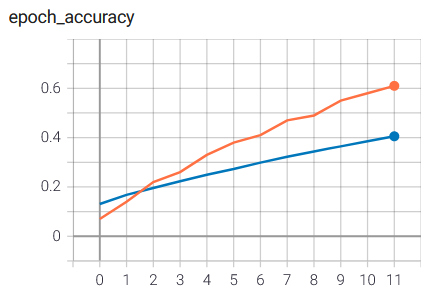
\includegraphics[width=0.49\textwidth]{TensorFlow/HistMNIST1acc}
		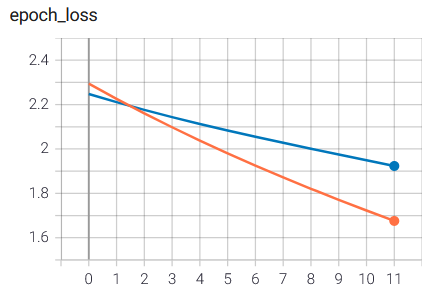
\includegraphics[width=0.49\textwidth]{TensorFlow/HistMNIST1loss}
		\caption{Trainingshistorie des einfachen Modells visualisiert mit TensorBoard} 
		\label{HistMNIST1}
	\end{center}
\end{figure}

\subsection{Probleme mit TensorBoard}
Bei der Verwendung von TensorBoard können Probleme bei dem Verbindungsaufbau, Laden der Daten oder Laden der 'richtigen' Daten auftreten.
Wenn zum Beispiel noch Daten angezeigt werden, die in der Zwischenzeit gelöscht wurden, oder aus einem anderen Grund ein komplettes Beenden
und Neustarten des TensorBoards erzwungen werden soll (manchmal kann es sich 'aufhängen'), können die folgenden Befehle - 
einzugeben im Windows command prompt - hilfreich sein:

\SHELL{taskkill /im tensorboard.exe /f}
\SHELL{del /q \%TMP\%\textbackslash.tensorboard-info\textbackslash*}

Es kann eine Fehlermeldung auftreten, dass die Datei nicht gefunden werden kann. Dies kann ignoriert werden. Nach kurzer Zeit sollte das TensorBoard
dann neu geladen werden können.

\subsection{Tieferes Netz}

Um das neuronale Netz \glqq intelligenter\grqq  zu machen, wird eine zusätzliche Schicht, eine \glqq hidden layer\grqq, hinzugefügt. 
Diese besteht aus 200 Neuronen mit der ReLu-Aktivierungsfunktion.
Eine weitere Verbesserung kann durch Dropout erzielt werden, die \glqq Overfitting\grqq, also das Auswendiglernen der Trainingsdaten, vermeidet.
Dies könnte auch durch eine wesentliche Erhöhung der Anzahl an Trainingsdaten erreicht werden, was aber natürlich auch eine wesentlich 
höhere Rechenzeit mit sich bringt. Stattdessen wird zwischen den beiden Schichten mit Neuronen eine Schicht eingefügt, die zufällig die Hälfte 
aller Informationen verwirft. Die neue Definition des Modells sieht wie folgt aus:

\begin{verbatim}
from tensorflow.keras.models import Sequential
from tensorflow.keras.layers import Dense,Flatten
from tensorflow.keras.layers import Dropout
model = Sequential()
model.add(Flatten())
model.add(Dense(200,activation='relu'))
model.add(Dropout(0.5))
model.add(Dense(10,activation='softmax'))
\end{verbatim}

Wie in Abbildung \ref{HistMNIST2} zu sehen ist, führt das Training mit dem tieferen Netz und Dropout zu besseren Ergebnissen.

\begin{figure}[H]
	\begin{center}
		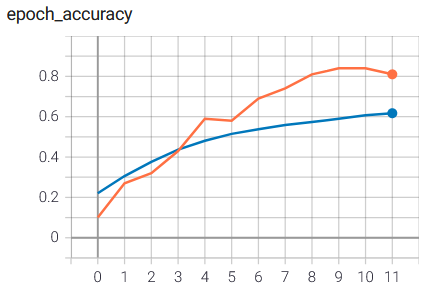
\includegraphics[width=0.49\textwidth]{TensorFlow/HistMNIST2acc}
		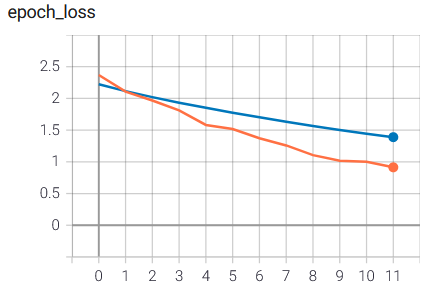
\includegraphics[width=0.49\textwidth]{TensorFlow/HistMNIST2loss}
		\caption{Trainingshistorie des einfachen Modells visualisiert mit TensorBoard} 
		\label{HistMNIST2}
	\end{center}
\end{figure}



\subsection{Convolutional Network}

Wie im Kapitel zu Convolutional Networks beschrieben, eignen sich diese besonders für Aufgaben der Bildklassifizierung.
Daher liegt der Gedanke natürlich nahe, sie auch hier zu verwenden. Dazu wird das Modell erneut neu definiert:

	
\begin{verbatim}
from tensorflow.keras.layers import Conv2D
from tensorflow.keras.layers import MaxPooling2D
model.add(Conv2D(
          32, kernel_size=(3, 3),
          activation='relu',
          input_shape=input_shape))
model.add(Conv2D(
          64, kernel_size=(3, 3),
          activation='relu'))
model.add(MaxPooling2D(
          pool_size=(2, 2)))
model.add(Dropout(0.25))
model.add(Flatten())
model.add(Dense(200,
activation = 'relu'))
model.add(Dropout(0.5))
model.add(Dense(10,
activation = 'softmax'))
\end{verbatim}




\medskip

In diesem Modell sind nun zwei Faltungsschichten und eine Pooling-Schicht zu finden.
Die neu hinzugefügten \PYTHON{Conv2D()}-Schichten gehören vor die bestehende Flatten()-Schicht, 
da sie die zweidimensionale Struktur der Eingabebilder nutzen. Die erste
Schicht lernt 32 Filter mit einer Matrixgröße von 3
x 3, die zweite 64 davon. Darauf folgt eine Maximum-Pooling-Schicht, die jeweils nur den größten Wert
von jedem $2 \times 2$-Feld speichert.

Mit dem auf 100 Samples begrenzten Trainingsdatensatz geht auch dieses Training noch fix. 
Die Historie ist in Abbildung \ref{HistMNIST3} abgebildet.

\begin{figure}[H]
	\begin{center}
		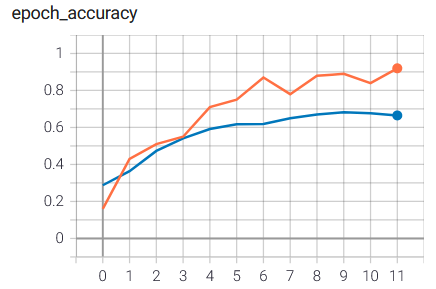
\includegraphics[width=0.49\textwidth]{TensorFlow/HistMNIST3acc}
		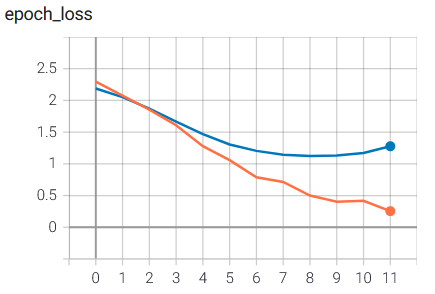
\includegraphics[width=0.49\textwidth]{TensorFlow/HistMNIST3loss}
		\caption{Trainingshistorie des einfachen Modells visualisiert mit TensorBoard} 
		\label{HistMNIST3}
	\end{center}
\end{figure}

Trainiert man über 12 Epochen mit allen 60.000 Trainingsdaten dauert das Training auf einem Laptop mit AMD Ryzen 5 3500U Prozessor
schon über 15 Minuten (ca. 1,5 Minuten je Epoche bei etwa 200ms pro Step). Dafür sind schon im sechsten (bzw. im fünften nach Notation in TensorBoard) 
Durchgang eine Genauigkeit von über 99 \% erreicht 
(siehe Abbildung \ref{HistMNIST3_60000}).

\begin{figure}[H]
	\begin{center}
		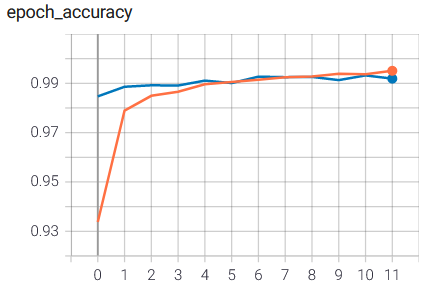
\includegraphics[width=0.49\textwidth]{TensorFlow/HistMNIST3acc_60000}
		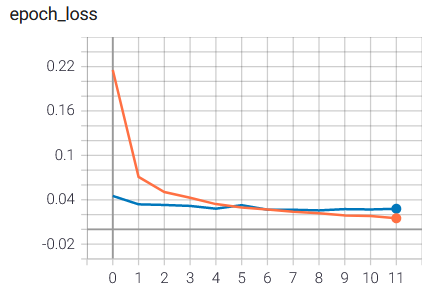
\includegraphics[width=0.49\textwidth]{TensorFlow/HistMNIST3loss_60000}
		\caption{Trainingshistorie des einfachen Modells visualisiert mit TensorBoard} 
		\label{HistMNIST3_60000}
	\end{center}
\end{figure}

\subsection{Vollständiger Code}
Der vollständige Code mit den zuvor beschriebenen Schritten (mit dem finalen CNN-Modell) ist untenstehend festgehalten.
Er wurde in Jupyter Notebook erstellt.

\lstinputlisting[language=Python, firstnumber=1]{../Code/JetsonNano/MNIST.py}
%\includepdf[pages=-]{MNIST.pdf}


%%%%%%%%%%%%%%%%%%%%%%%%%%%%%%%%%%%%%%%%%%%%%%%%%%%%%%%%%%%%         nächstes Tutorial

\section{\glqq Hello World 2\grqq - Erkenung einer Iris}

Die Erkennung der Iris (Schwertlilie) ist ein weiterer Klassiker zur Bildklassifizierung. Auch zu diesem Klassiker gibt es mehrere Tutorials.
Die folgende Anleitung orientiert sich an dem Tutorial von \cite{KDnuggets.07.12.2020}.

Ziel dieses Tutorials ist die Klassifizierung dreier verschiedener Iris-Arten anhand der Länge und Breite von Kelchblatt (sepal) und Blütenblatt (petal).

\subsection{Laden der Daten und Bibliotheken}
Der Datensatz \glqq Iris\grqq{} wird mit der Bibliothek \PYTHON{sklearn} ausgeliefert.

\begin{verbatim}
from sklearn.datasets import load_iris
iris = load_iris()
\end{verbatim}

Für die Bilderkennung müssen wietere Bibliotheken geladen werden:

\begin{verbatim}
import numpy as np
import pandas as pd
import matplotlib.pyplot as plt

import tensorflow as tf
from tensorflow.keras.models import Sequential
from tensorflow.keras.layers import Dense
\end{verbatim}


Die Bibliotheken numpy, pandas und pyplot werden für die Vorbereitung und Visualisierung der Daten sowie Ergebnisse verwendet.

In einem neuronalen Netz werden die Berechnungen sequentiell abgearbeitet. Passend dazu
wird der Modelltype \PYTHON{Sequential} importiert. Das Modell wird aus einzelnen
Schichten aufgebaut, die sequentiell bearbeitet werden. Der Schichttyp \PYTHON{Dense}
wird anschließend importiert. Der Schichttyp  ist eine Art von Schicht, die \glqq dicht\grqq{} 
verbunden ist, was bedeutet, dass alle Knoten der vorherigen Schicht mit allen Knoten der 
aktuellen Schicht verbunden sind.

\subsection{Der Datensatz}
Der Datensatz ist ein \PYTHON{dictionary}. Seine Schlüssel
kann man sich leicht anzeigen lassen:

\begin{verbatim}
>>> iris.keys()
\end{verbatim}


als Output erhält man:

\begin{lstlisting}[numbers=none]
dict\_keys(['data', 'target', 'frame', 'target\_names', 'DESCR', 'feature\_names', 'filename'])
\end{lstlisting}
\medskip

Die einzelnen Elemente kann man sich nun ansehen.
Nach Eingabe des Befehls 
\begin{verbatim}
iris['DESCR']
\end{verbatim}
wird eine ausführliche Beschreibung ausgegeben:


\begin{lstlisting}[numbers=none]
'.. _iris_dataset:

Iris plants dataset
--------------------

**Data Set Characteristics:**

    :Number of Instances: 150 (50 in each of three classes)    
    :Number of Attributes: 4 numeric, predictive attributes and the class
    :Attribute Information:
        - sepal length in cm
        - sepal width in cm
        - petal length in cm
        - petal width in cm
        - class:
                - Iris-Setosa
                - Iris-Versicolour
                - Iris-Virginica
                
    :Summary Statistics:
    
    ============== ==== ==== ======= ===== ====================
                    Min  Max   Mean    SD   Class Correlation
    ============== ==== ==== ======= ===== ====================
    sepal length:   4.3  7.9   5.84   0.83    0.7826
    sepal width:    2.0  4.4   3.05   0.43   -0.4194
    petal length:   1.0  6.9   3.76   1.76    0.9490  (high!)
    petal width:    0.1  2.5   1.20   0.76    0.9565  (high!)
    ============== ==== ==== ======= ===== ====================
    
    :Missing Attribute Values: None
    :Class Distribution: 33.3% for each of 3 classes.
    :Creator: R.A. Fisher
    :Donor: Michael Marshall (MARSHALL%PLU@io.arc.nasa.gov)
    :Date: July, 1988
    
The famous Iris database, first used by Sir R.A. Fisher. The dataset is taken
from Fisher\'s paper. Note that it\'s the same as in R, but not as in the UCI
Machine Learning Repository, which has two wrong data points.

This is perhaps the best known database to be found in the
pattern recognition literature.  Fisher\'s paper is a classic in the field and
is referenced frequently to this day.  (See Duda & Hart, for example.)  The
data set contains 3 classes of 50 instances each, where each class refers to a
type of iris plant.  One class is linearly separable from the other 2; the
latter are NOT linearly separable from each other.

.. topic:: References
   - Fisher, R.A. "The use of multiple measurements in taxonomic problems"
     Annual Eugenics, 7, Part II, 179-188 (1936); also in "Contributions to
     Mathematical Statistics" (John Wiley, NY, 1950).
   - Duda, R.O., & Hart, P.E. (1973) Pattern Classification and Scene Analysis.
     (Q327.D83) John Wiley & Sons.  ISBN 0-471-22361-1.  See page 218.
   - Dasarathy, B.V. (1980) "Nosing Around the Neighborhood: A New System
     Structure and Classification Rule for Recognition in Partially Exposed
     Environments".  IEEE Transactions on Pattern Analysis and Machine
     Intelligence, Vol. PAMI-2, No. 1, 67-71.
   - Gates, G.W. (1972) "The Reduced Nearest Neighbor Rule".  IEEE Transactions
     on Information Theory, May 1972, 431-433.
   - See also: 1988 MLC Proceedings, 54-64.  Cheeseman et al"s AUTOCLASS II
     conceptual clustering system finds 3 classes in the data.
   - Many, many more ...'
\end{lstlisting}

Mit der Eingabe

\begin{verbatim}
iris['feature_names']
\end{verbatim}

wird klar, dass die Eigenschaften, anhand derer die Blumen klassifiziert werden, die Länge und Breite des Kelchblatts (sepal) und Blütenblatts (petal) sind:

\begin{lstlisting}[numbers=none]
['sepal length (cm)',
 'sepal width (cm)',
 'petal length (cm)',
 'petal width (cm)']
\end{lstlisting}

Die Namen der Blumen, die nach der Eingabe
\begin{verbatim}
iris['target_names']
\end{verbatim}

angezeigt werden, sind

\begin{lstlisting}[numbers=none]
array(['setosa', 'versicolor', 'virginica'], dtype='<U10')
\end{lstlisting}

Zur weiteren Untersuchung werden die Daten mit den Überschriften in einen Datenrahmen aufgenommen.

\begin{verbatim}
X = pd.DataFrame(data = iris.data, columns = iris.feature_names)
print(X.head())
\end{verbatim}

Der Befehl \PYTHON{(X.head())} zeigt - wie in Abbildung~\ref{TensorFlowHead} den Kopf des Datenrahmens an.
Ersichtlich ist, dass jeder Datensatz aus vier Werten besteht. 

\begin{figure}[H]
	\GRAPHICSC{0.6}{1.0}{TensorFlow/IrisHead}
	\caption{Kopfzeilen des Datensatzes Iris}\label{TensorFlowHead}
\end{figure}

Jeder Datensatz enthält auch schon in dem Schlüssel \PYTHON{target} seine Klassifikation. In der 
Abbildung~\ref{TensorFlowHeadType} ist dies für die ersten Datensätze aufgeführt.

\begin{verbatim}
y = pd.DataFrame(data=iris.target, columns = ['irisType'])
y.head()
\end{verbatim}

\begin{figure}[H]
	\GRAPHICSC{1.0}{1.0}{TensorFlow/IrisHeadType}
	\caption{Ausgabe der Kategorien des Datensatzes Iris}\label{TensorFlowHeadType}
\end{figure}

Mittels des Befehls 
\begin{verbatim}
y.irisType.value_counts()
\end{verbatim}



kann ermittel werden,
wie viele Klassen vorliegen. Die Ausgabe des Befehls wird in der Abbildung~\ref{TensorFlowIrisTypes}
gezeigt; es ergeben sich 3 Klassen mit den Nummern $0$, $1$ und $2$. Jeweils 50 Datensätze sind ihnen zugeordnet.

\begin{figure}[H]
	\GRAPHICSC{1.0}{1.0}{TensorFlow/IrisTypes}
	\caption{Namen der Kategorien im Datensatz Iris}\label{TensorFlowIrisTypes}
\end{figure}


\subsection{Datenvorbereitung}
Nun kann der Prozess gestartet werden. Zunächst müssen die Daten vorbereitet werden.
In diesem Fall sind folgende Schritte notwendig: 

\begin{enumerate}
  \item Fehlende Werte müssen ergänzt werden.
  \item Die Daten müssen in Trainings- und Validierungsdaten aufgeteilt werden.
  \item Die Daten werden normalisiert.
  \item Die Daten, die Kategorien darstellen, müssen in einen Vektor umgewandelt werden.
  \item Die Daten werden in Vektoren eingetragen.
\end{enumerate}
	
\subsubsection{1. Fehlende Werte}

Mit dem Befehl 
\begin{verbatim}
pandas.DataFrame.info()
\end{verbatim}
 kann geprüft werden, ob die Daten
konsistent sind. Die Abbildung~\ref{TensorFlowIrisInfo} zeigt, dass die Daten vollständig sind und
der Datentype für alle Werte identisch ist. Demzufolge existiert für diesen Datensatz kein Handlungsbedarf.

\begin{verbatim}
X.info()
\end{verbatim}

\begin{figure}[H]
	\GRAPHICSC{1.0}{1.0}{TensorFlow/IrisInfo}
	\caption{Prüfung des Datensatzes Iris}\label{TensorFlowIrisInfo}
\end{figure}


\subsubsection{2. Aufteilung in Trainigs- und Validierungsdaten}

Zur Aufteilung eines Datensatzes  in Trainings- und Validierungsdaten steht in der Bibliothek
\PYTHON{sklearn} in der Klasse \PYTHON{model\_selection} die Methode \PYTHON{train\_test\_split}
zur Verfügung. Hier werden 10\% des Datensatzes als Validierungsdaten zurückgehalten.

\begin{verbatim}
X_train, X_test, y_train, y_test = train_test_split(X,y, test_size=0.1)
\end{verbatim}

\subsubsection{3. Normalisierung der Daten}

Falls die Daten eine hohe Varianz haben, so sind sie zu normalisieren. Daher wird zuerst die Varianz ermittelt.
Die Funktion \PYTHON{var()} steht dafür aus der Klasse \PYTHON{pandas.DataFrame} zur Verfügung. Die Ausgabe zeigt
gemäß Abbildung~\ref{TensorFlowIrisVar}, dass die Varianz gering ist und somit kein Handlungsbedarf besteht.

\begin{verbatim}
X_train.var(), X_test.var()
\end{verbatim}


\begin{figure}[H]
	\GRAPHICSC{1.0}{1.0}{TensorFlow/IrisVariance}
	\caption{Varianz im Datensatzes Iris}\label{TensorFlowIrisVar}
\end{figure}

\subsubsection{4. Konvertierung der Kategorien in einen Vektor}

Aus der Untersuchung des Datensatzes ist bekannt, dass drei Kategorien enthalten sind. Derzeit sind
sie mit $0$, $1$ und $2$ nummeriert. Der verwendete Algorithmus könnte höhere Werte eine höhere Priorität 
zuordnen, so dass das Ergebnis verzerrt wird. Um dies zu vermeiden, wird ein Vektor generiert, der nur die
Wert $0$ und $1$ enthält und die Kategrie somit kodiert. Dies ist ein sogenannter \glqq OneHotVector\grqq{}.
Dazu liegen zwei Möglichkeiten vor. Einmal könnte die Funktion \PYTHON{to\_categorical} der Bibliothek
\PYTHON{Keras} verwendet werden oder die Funktion \PYTHON{OneHotEncoder} der Bibliothek \PYTHON{sklearn}.



\begin{verbatim}
y_train = tf.keras.utils.to_categorical(y_train)
y_test = tf.keras.utils.to_categorical(y_test)
\end{verbatim}

\bigskip

Das Ergebnis der ersten fünf Daten zeigt die Abbildung~\ref{TensorFlowIrisCat} auf der rechten Seite. Es wird angezeigt mit

\begin{verbatim}
y_train[:5,:]
\end{verbatim}

Auf der linken Seite der Abbildung ist die ursprüngliche Codierung der Kategorien angezeigt. Hier ist auch zu sehen, welche Datensätze zufällig als die ersten fünf
Trainingsdaten ausgewählt wurden.

\begin{figure}[H]
	\begin{center}
		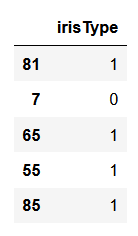
\includegraphics[width=0.2\textwidth]{TensorFlow/IrisCat1}
		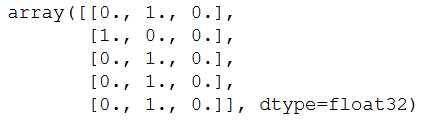
\includegraphics[width=0.6\textwidth]{TensorFlow/IrisCat}
		\caption{Codierung der Kategorien vor (links) und nach der Konvertierung} 
		\label{TensorFlowIrisCat}
	\end{center}
\end{figure}



\subsubsection{5. Konvertierung der Daten in Vektoren}

Damit die Daten einfacher weiterverarbeitet werden können, werden sie noch in Vektoren der 
Bibliothek \PYTHON{numpy} umgewandelt.

\begin{verbatim}
X_train = X_train.values
X_test = X_test.values
\end{verbatim}

Das Ergebnis der Konvertierung kann im ersten Datensatz geprüft werden:

\begin{verbatim}
X_train[0]
\end{verbatim}

Das Ergebnis sieht wie folgt aus:

\begin{lstlisting}[numbers=none]
array([5.5, 2.4, 3.7, 1. ])
\end{lstlisting}


\subsection{Modell für das Maschinelle Lernen}

Nach den Vorbereitungen kann nun das sequentielle Modell erstellt werden und die Schichten hinzugefügt werden.

\begin{verbatim}
model1 = Sequential()
model1.add(Dense(64,activation='relu', input_shape= X_train[0].shape))
model1.add(Dense(128,activation='relu'))
model1.add(Dense(128,activation='relu'))
model1.add(Dense(128,activation='relu'))
model1.add(Dense(128,activation='relu'))
model1.add(Dense(64,activation='relu'))
model1.add(Dense(64,activation='relu'))
model1.add(Dense(64,activation='relu'))
model1.add(Dense(64,activation='relu'))
model1.add(Dense(3,activation='softmax'))
\end{verbatim}

In diesem Beispiel
besteht das Model aus einer Eingabeschicht, acht versteckten Schichten und einer 
Ausgabeschicht. Die Aktivierungsfunktion der ersten Schichten ist die \PYTHON{relu}, nur für die Ausgabeschicht
wird die Aktivierungsfunktion \PYTHON{softmax} verwendet, da diese den möglichen Kategorien Wahrscheinlichkeiten
zuweist. Für den Fall, dass nur zwei mögliche Kategorien vorliegen, würde man die Aktivierungsfunktion
\PYTHON{sigmoid} wählen. Neben der Aktiverungsfunktion \PYTHON{relu} stehen auch die Funktionen \PYTHON{sigmoid}, \PYTHON{linear}
oder \PYTHON{tanh} zur Wahl. Die Experimente haben gezeigt, dass die Aktivierungsfunktion \PYTHON{relu}
den besten Erfolg zeigt.

Die Eingabeschicht enthält ein zusätzliches Argument \PYTHON{input\_shape}. Dieses Argument sorgt, dafür, dass die
Dimension der ersten Schicht sich an der Dimension eines Datensatzes orientiert. In diesem Beispiel
ist die Größe vier.

Im nächsten Schritt wird nun das Modell fertiggestellt. Dazu muss der Optimierung, die Bewertungsfunktion und die Metrik übergeben werden.

\begin{verbatim}
model1.compile(optimizer='adam', loss= 'categorical_crossentropy', metrics = ['acc'])
\end{verbatim}

Für die Optimierungsfunktion stehen mehrere Kandidaten zur Verfügung:
\PYTHON{Stochastic Gradient Descent}, \PYTHON{RMSProp} oder auch \PYTHON{adam}. Hier wurde
wie auch im vorherigen Beispiel Adam verwendet.

Für die Bewertungsfunktion wird hier \PYTHON{categorical\_crossentropy} verwendet, die meistens in 
Klassifizierungsaufgaben mit mehreren Klassen verwendet wird, bei denen jeweils nur eine Kategorie richtig ist. 
Falls nur zwei
Kategorien zur Verfügung stehen, so wird stattdessen \PYTHON{binary\_crossentropy} verwendet.

Metriken sind wichtig, um das eigene Modell zu bewerten. Es gibt verschiedene Metriken, 
anhand derer wir unser Modell bewerten können. Bei Klassifizierungsproblemen ist die 
wichtigste Metrik die Genauigkeit \PYTHON{['acc']}, die angibt, wie genau unsere Vorhersagen sind.

Im letzten Schritt wird das Modell nun anhand der Trainingsdaten trainiert.

\begin{verbatim}
history = model1.fit(X_train, y_train, batch_size = 40, epochs=800, validation_split = 0.1)
\end{verbatim}

Für die Erstellung des Modells wurden hier 800 Epochen mit einer Batchgröße 40 eingestellt. Als Validierungsdaten werden zufällig 
10\% des Trainingsdatensatzes entnommen.

\subsection{Historie}

Die Methode \PYTHON{fit} gibt eine Datenstruktur zurück, die die gesamte Geschichte unseres Trainings enthält. So kann verfolgt werden, 
wie sich die Qualität während des Trainings entwickelt hat. Zum Beispiel kann durch wesentlich bessere Performance in den Trainingsdaten als in den
Validierungsdaten ein Hinweis auf Overfitting entdeckt werden. Außerdem kann man sehen, ob die Qualität sich in den letzten Epochen asymptotisch verhält oder
das Training verlängert werden sollte oder verkürzt werden kann.\\

Der Rückgabewert ist ein Dictionary, auf das mittels \PYTHON{history.history} zugegriffen werden kann.
 Hier kann man unter anderem  die Entwicklung der Genauigkeit im Trainings- als auch im Validierungsdatensatz
verfolgen. Auf die Historie der Elemente acc, loss, val\_loss und val\_acc können wir je mit history.history.loss oder history.history['val\_acc'] usw. zugreifen.


In der Abbildung~\ref{TensorFlowIrisPlotHist1}
ist der Verlauf der Genauigkeit über die Epochen dargestellt. Für die Erzeugng des Graphen sind nur fünf Zeilen 
zu programmieren:

\begin{verbatim}
plt.plot(history.history['acc'])
plt.plot(history.history['val_acc'])
plt.xlabel('Epochs')
plt.ylabel('Acc')
plt.legend(['Training', 'Validation'], loc='upper right')
\end{verbatim}

\begin{figure}[H]
	\GRAPHICSC{0.8}{1.0}{TensorFlow/IrisPlotHist1}
	\caption{Verlauf der Genauigkeit für die Trainings- und Testdaten während des Trainings des Modells}\label{TensorFlowIrisPlotHist1}
\end{figure}

Analog kann der Verlauf der  Verlustfunktion gezeichnet werden:

\begin{verbatim}
plt.plot(history.history['loss'])
plt.plot(history.history['val_loss'])
plt.xlabel('Epochs')
plt.ylabel('Loss')
plt.legend(['Training', 'Validation'], loc='upper left')
\end{verbatim}

\begin{figure}[H]
	\GRAPHICSC{0.7}{1.0}{TensorFlow/IrisPlotHist2}
	\caption{Verlauf der Verlustfunktion für die Trainings- und Testedaten während des Trainings des Modells}\label{TensorFlowIrisPlotHist2}
\end{figure}

Laut \cite{KDnuggets.07.12.2020} erwarten wir ein Overfitting zu beobachten, was sich darin äußert, dass die Ergebnisse für die Trainingsdaten
deutlich besser sind als für die Validierungsdaten. In den erzielten Ergebnissen jedoch ist dieses Problem nicht zu erkennen. Die Validierungsdaten
schneiden sogar besser ab als die Trainingsdaten. Vergleichen Sie dazu auch mit den Plots von \cite{KDnuggets.07.12.2020}. Eventuell wurden hier
unterschiedliche Versionen von TensorFlow verwendet, die zu unterschiedlichen Ergebnissen führen.

Zur Überprüfung des Modells kann die Funktion  \PYTHON{model.evaluate} verwendet werden; die
Methode erwartet die Testdaten mit den zugehörigen Kategorien:

\begin{verbatim}
model1.evaluate(X_test, y_test)
\end{verbatim}

Die erreichte Genauigkeit auf die Testdaten liegt bei etwa 87 \%.


\subsection{Regularisierung}

Um ein besseres Modell zu erreichen, wird eine Regularisierung eingeführt. Dies reduziert die Gefahr des Overfittings
(welches für das erste Modell erwartet wurde). In diesem Modell wird eine L2-Regularisierung hinzugefügt. 
Diese fügt in der Verlustfunktion zur Ermittlung der Gewichte den quadrierten Betrag des jeweiligen Koeffizienten als Strafterm hinzu.  

Als zweite Maßnahme zur Reduzierung des Overfittings und der Verbesserung des Modells, werden Dropout-Schichten hinzugefügt.


\begin{verbatim}
model2 = Sequential()
model2.add(Dense(64, activation = 'relu', input_shape= X_train[0].shape))
model2.add(Dense(128, activation = 'relu', kernel_regularizer=tf.keras.regularizers.l2(0.001)))
model2.add(Dense (128, activation = 'relu',kernel_regularizer=tf.keras.regularizers.l2(0.001)))
model2.add(tf.keras.layers.Dropout(0.5))
model2.add(Dense (128, activation = 'relu', kernel_regularizer=tf.keras.regularizers.l2(0.001)))
model2.add(Dense(128, activation = 'relu', kernel_regularizer = tf.keras.regularizers.l2(0.001)))
model2.add(Dense (64, activation = 'relu', kernel_regularizer=tf.keras.regularizers.l2(0.001)))
model2.add(Dense (64, activation = 'relu', kernel_regularizer=tf.keras.regularizers.l2(0.001)))
model2.add(tf.keras.layers.Dropout(0.5))
model2.add(Dense (64, activation = 'relu', kernel_regularizer=tf.keras.regularizers.l2(0.001)))
model2.add(Dense (64, activation = 'relu', kernel_regularizer=tf.keras.regularizers.l2(0.001)))
model2.add(Dense (3, activation = 'softmax', kernel_regularizer=tf.keras.regularizers.l2(0.001)))
\end{verbatim}

Neben der Einführung der Regularisierung und der zwei Dropout-Schichten wird im Modell  und an den Parametern
nichts geändert. 

\begin{verbatim}
model2.compile(optimizer='adam', loss='categorical_crossentropy', metrics=['acc'])
history2 = model2.fit(X_train, y_train, epochs=800, validation_split=0.1, batch_size=40)
model2.evaluate(X_test, y_test)
\end{verbatim}

Auch für dieses Modell wird eine Genauigkeit von 87 \% anhand der Testdaten erreicht.

Den Verlauf der Genauigkeit und der Bewertungsfunktion werden in den Abbildungen \ref{TensorFlowIrisPlotHist3}
und \ref{TensorFlowIrisPlotHist4} gezeigt. 


\begin{verbatim}
plt.plot(history2.history['acc'])
plt.plot(history2.history['val_acc'])
plt.title('Accuracy vs. epochs')
plt.ylabel('Acc')
plt.xlabel('Epoch')
plt.legend(['Training', 'Validation'], loc='lower right')
plt.show()
\end{verbatim}


\begin{figure}[H]
	\GRAPHICSC{0.8}{1.0}{TensorFlow/IrisPlotHist3}
	\caption{Verlauf der Genauigkeit für die Trainings- und Testdaten während des Trainings des zweiten Modells}
	\label{TensorFlowIrisPlotHist3}
\end{figure}


Der Python-Programmteil für die Verlustfunktion ist wie folgt gegeben:

\begin{verbatim}
plt.plot(history2.history['loss'])
plt.plot(history2.history['val_loss'])
plt.title('Loss vs. epochs')
plt.ylabel('Loss')
plt.xlabel('Epoch')
plt.legend(['Training', 'Validation'], loc='upper right')
plt.show()
\end{verbatim}

\begin{figure}[H]
	\GRAPHICSC{0.8}{1.0}{TensorFlow/IrisPlotHist4}
	\caption{Verlauf der Verlustfunktion für die Trainings- und Testdaten während des Trainings des zweiten Modells}
	\label{TensorFlowIrisPlotHist4}
\end{figure}

\subsection{Vollständiger Code}
Nachfolgend ist das gesamte Skript des beschriebenen Tutorials, als Jupyter Notebook, zu finden:

\lstinputlisting[language=Python, firstnumber=1]{../Code/JetsonNano/Iris.py}




\section{Sichern und Wiederherstellen eines Modells}
Ein Tutorial zum Sichern und Laden eines Modells oder seiner Gewichte ist zu finden unter \url{https://www.tensorflow.org/tutorials/keras/save_and_load}.

\subsection{Setup}
Um Modelle im HDF5 Format speichern zu können, ist zunächst eine Installation notwendig (im Anaconda prompt):

\medskip

\SHELL{pip install -q pyyaml h5py}

\medskip

Außerdem importieren wir zu Beginn des Codes das Operating System Interface und Keras:

\begin{verbatim}
import os

import tensorflow as tf
from tensorflow import keras
\end{verbatim}

\subsection{Checkpoints während des Trainings}

Mit Callbacks können die Gewichte während des Trainings gespeichert werden. 
Dadurch wird eine einzelne Sammlung von TensorFlow-Prüfpunktdateien erstellt, die am Ende jeder Epoche aktualisiert werden.
Dazu wird zuerst eine Checkpoint-Datei angelegt:

\begin{verbatim}
checkpoint_path = "training_1/cp.ckpt"
checkpoint_dir = os.path.dirname(checkpoint_path)
\end{verbatim}

Es ist auch möglich, die Kontrollpunkte eindeutig anhand der Epoche zu benennen, dann ändert sich die Eingabe zu

\begin{verbatim}
checkpoint_path = "training_2/cp-{epoch:04d}.ckpt"
checkpoint_dir = os.path.dirname(checkpoint_path)
\end{verbatim}

Danach wird der Callback angelegt: 
\begin{verbatim}
# Create a callback that saves the model's weights
cp_callback = tf.keras.callbacks.ModelCheckpoint(
	filepath=checkpoint_path,
		save_weights_only=True,
		verbose=1)
\end{verbatim}

Sollen die Gewichte nur alle beispielsweise 5 Epochen gespeichert werden, wird der Callback wie folgt angelegt:
\begin{verbatim}
# Create a callback that saves the model's weights every 5 epochs
cp_callback = tf.keras.callbacks.ModelCheckpoint(
    filepath=checkpoint_path, 
    verbose=1, 
    save_weights_only=True,
    save_freq=5*batch_size)

# Save the weights using the `checkpoint_path` format
model.save_weights(checkpoint_path.format(epoch=0))
\end{verbatim}

Um die Gewichte im Training zu speichern muss der Callback dann
noch der Funktion \PYTHON{model.fit()} übergeben werden:

\begin{verbatim}
# Train the model with the new callback
model.fit(train_images, 
          train_labels,  
          epochs=10,
          validation_data=(test_images, test_labels),
          callbacks=[cp_callback])  # Pass callback to training
\end{verbatim}

Es kann sein, dass auf diesem Wege eine Warnmeldung generiert wird, die aber ignoriert werden kann.

Zwischen zwei Modellen mit derselben Architektur können die Gewichte mit Hilfe der erstellten Checkpoint-Datei geteilt werden.
Sei \PYTHON{model} ein zweites Modell mit der gleichen Architektur wie das Modell, deren Gewichte gespeichert wurden,
lädt man die Gewichte aus dem Checkpoint wie folgt in das neue Modell:

\begin{verbatim}
model.load_weights(checkpoint_path)
\end{verbatim}

\subsection{Manuelles Speichern von Gewichten}
Das manuelle Speichern von Gewichten erfolgt mit
\begin{verbatim}
model.save_weights('./checkpoints/my_checkpoint')
\end{verbatim}
Standardmäßig wird so mit der Erweiterung .ckpt gespeichert.

\subsection{Speichern des gesamten Modells}

Über die Funktion \PYTHON{model.save} können Architektur, Gewichte und Trainingskonfiguration eines Modells in einer einzigen Datei gespeichert werden. 
Es gibt zwei Dateiformate, um ein gesamtes Modell zu speichern. Standard in TensorFlow 2 ist SavedModel. Es ist aber auch möglich, Modelle
im Format HDF5 zu speichern.

  

\subsubsection{SavedModel-Format}
Das Speichern im SavedModel-Format erfolgt in nur zwei Zeilen.

\begin{verbatim}
!mkdir -p saved_model
model.save('saved_model/my_model')
\end{verbatim}

Das Modell kann daraufhin aus dem gespeicherten Modell neu geladen werden:

\begin{verbatim}
new_model = tf.keras.models.load_model('saved_model/my_model')
\end{verbatim}

\subsubsection{HDF5-Format}
Um das Modell im HDF5-Format zu speichern, wird die entsprechende Endung angegeben. Es ist nur eine Zeile notwendig:

\begin{verbatim}
model.save('my_model.h5')
\end{verbatim}

Geladen wird das Modell entsprechend mit dem Dateinamen inklusive der h5-Endung:

\begin{verbatim}
new_model = tf.keras.models.load_model('my_model.h5')
\end{verbatim}

\section{Optimizing Training Time Performance}

Auf der Website 
\url{https://www.kdnuggets.com/2020/03/tensorflow-optimizing-training-time-performance.html}
findet sich ein TensorFlow 2.0 Tutorial zur Optimierung der Trainingszeit.
Dazu stehen verschiedene Ansatzpunkte zur Verfügung:

\begin{enumerate}
\item f.data
\item Mixed Precision Training
\item Multi-GPU Training Strategy
\end{enumerate}
Insgesamt soll so das Training um bis zu $2-10 \times$ beschleunigt werden können. \cite{KDnuggets.11.12.2020}
 
\subsection{Engpass identifizieren}
Bei Verwendung einer Nvidia-Karte ist die einfachste Lösung zur Überwachung der GPU-Auslastung über die Zeit wahrscheinlich 
\SHELL{nvtop}. Ein möglicher Output ist in Abbildung \ref{Fignvtop} zu sehen 

\begin{figure}[H]
	\begin{center}
		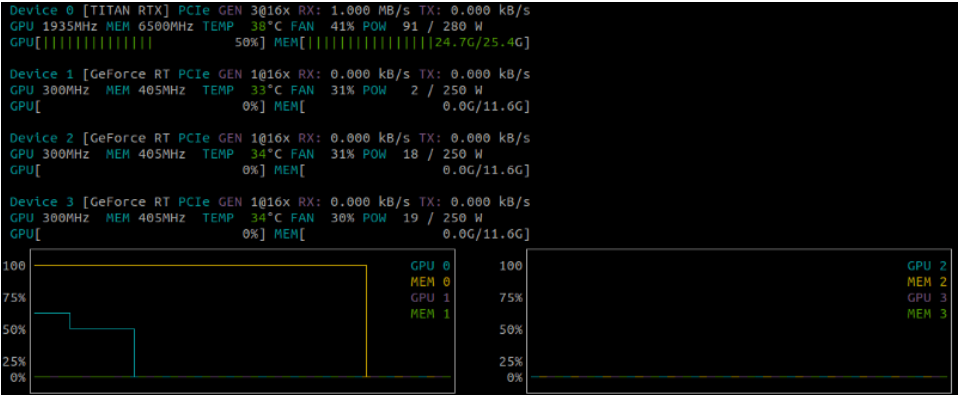
\includegraphics[width=0.9\textwidth]{TensorFlow/nvtop}
		\caption{Visualisierung von Engpässung mit \SHELL{nvtop} Quelle:\cite{KDnuggets.11.12.2020}} 
		\label{Fignvtop}
	\end{center}
\end{figure}

Zur Visualisierung der Auslastung mit TensorBoard muss nur

\begin{verbatim}
profile_batch={BATCH_INDEX_TO_MONITOR}
\end{verbatim}

im TensorBoard Callback hinzugefügt werden. Dann wird ein vollständiger Bericht über die Operationen erstellt, die 
entweder von der CPU oder der GPU für den gegebenen Batch durchgeführt wurden. 
Dies kann dabei helfen, zu erkennen, ob die GPU an einem bestimmten Punkt aufgrund fehlender Daten blockiert ist.

\begin{figure}[H]
	\begin{center}
		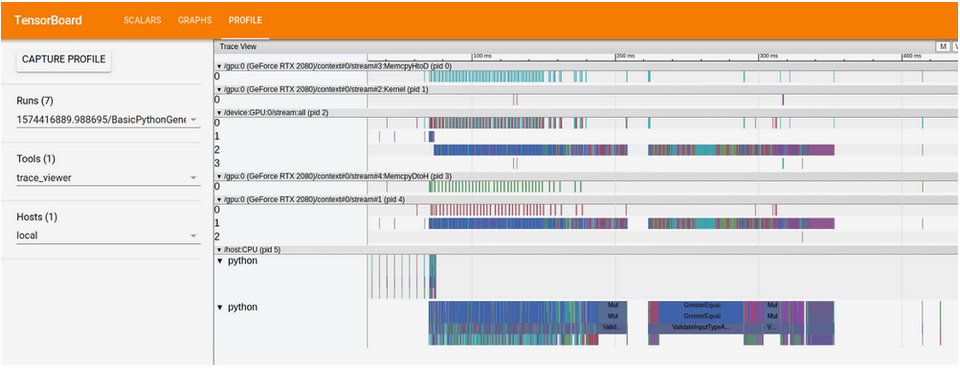
\includegraphics[width=0.9\textwidth]{TensorFlow/TensorBoardBottleneck}
		\caption{Visualisierung von Engpässung mit TensorBoard Quelle:\cite{KDnuggets.11.12.2020}} 
		\label{TensorBoardBottleneck}
	\end{center}
\end{figure}




\subsection{tf.data}
Um die GPU durchgängig arbeiten zu lassen, muss der Engpass des Datenladens beseitigt werden. 
In Abbildung \ref{TensorBoardBottleneckData} ist zu erkennen, dass die GPU nicht arbeitet, 
während die CPU mit dem Laden von Daten beschäftigt ist.

\begin{figure}[H]
	\begin{center}
		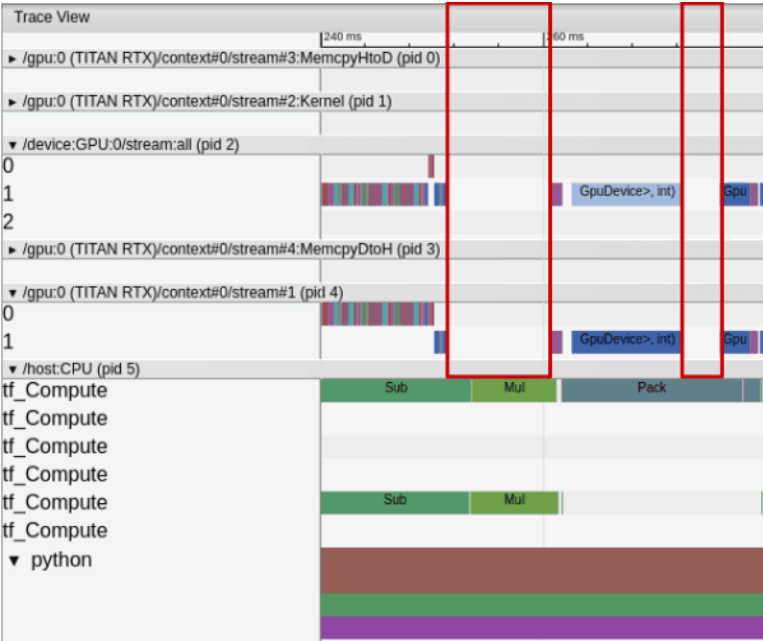
\includegraphics[width=0.9\textwidth]{TensorFlow/TensorBoardBottleneckData}
		\caption{Bottleneck Daten laden Quelle:\cite{KDnuggets.11.12.2020}} 
		\label{TensorBoardBottleneckData}
	\end{center}
\end{figure}

Als erstes sollte zur Beseitigung dieses Engpasses vom Keras sequences
zu tf.data gewechselt werden. Danach können weitere Optimierungen vorgenommen werden:


\begin{enumerate}
\item Parallelisierung: Mit \PYTHON{num\_parallel\_calls\=tf.data.experimental.AUTOTUNE} werden die \PYTHON{.map()} calls parallelisiert
\item Cache: Geladene Bilder im Speicher halten durch Zwischenspeichern von Datensätzen vor der Patch-Auswahl
\item Prefetching: Start des Abrufs von Elementen, bevor der vorherige Batch beendet ist
\end{enumerate}

Im folgenden ist beispielhaft ein optimierter Code zur Datensatz-Erstellung mit scharfen und verschwommenen Bildern zu sehen:

\begin{verbatim}[frame=single]
#dataset creation for optimizing training time
#from https://www.kdnuggets.com/2020/03/tensorflow-optimizing-training-time-performance.html

from pathlib import Path

import tensorflow as tf

def select_patch(sharp, blur, patch_size_x, patch_size_y):
    """
    Select a patch on both sharp and blur images at the same localization.
    Args:
        sharp (tf.Tensor): Tensor for the sharp image
        blur (tf.Tensor): Tensor for the blur image
        patch_size_x (int): Size of patch along x axis
        patch_size_y (int): Size of patch along y axis
    Returns:
        Tuple[tf.Tensor, tf.Tensor]: Tuple of tensors with shape (patch_size_x, patch_size_y, 3)
    """
    stack = tf.stack([sharp, blur], axis=0)
    patches = tf.image.random_crop(stack, size=[2, patch_size_x, patch_size_y, 3])
    return (patches[0], patches[1])


class TensorflowDatasetLoader:
    def __init__(self, dataset_path, batch_size=4, patch_size=(256, 256), n_epochs=10, n_images=None):
        # List all images paths
        sharp_images_paths = [str(path) for path in Path(dataset_path).glob("*/sharp/*.png")]
        if n_images is not None:
            sharp_images_paths = sharp_images_paths[0:n_images]

        # Generate corresponding blurred images paths
        blur_images_paths = [path.replace("sharp", "blur") for path in sharp_images_paths]

        # Load sharp and blurred images
        sharp_dataset = tf.data.Dataset.from_tensor_slices(sharp_images_paths).map(
            lambda path: self.load_image(path, dtype),
            num_parallel_calls=tf.data.experimental.AUTOTUNE,
        )
        blur_dataset = tf.data.Dataset.from_tensor_slices(blur_images_paths).map(
            lambda path: self.load_image(path, dtype),
            num_parallel_calls=tf.data.experimental.AUTOTUNE,
        )

        dataset = tf.data.Dataset.zip((sharp_dataset, blur_dataset))
        dataset = dataset.cache()

        # Select the same patch on the sharp image and its corresponding blurred
        dataset = dataset.map(
            lambda sharp_image, blur_image: select_patch(
                sharp_image, blur_image, patch_size[0], patch_size[1]
            ),
            num_parallel_calls=tf.data.experimental.AUTOTUNE,
        )

        # Define dataset characteristics (batch_size, number_of_epochs, shuffling)
        dataset = dataset.batch(batch_size)
        dataset = dataset.shuffle(buffer_size=50)
        dataset = dataset.repeat()
        dataset = dataset.prefetch(buffer_size=tf.data.experimental.AUTOTUNE)

        self.dataset = dataset

    @staticmethod
    def load_image(image_path, dtype):
        image = tf.io.read_file(image_path)
        image = tf.image.decode_png(image, channels=3)
        image = tf.image.convert_image_dtype(image, dtype)
        image = (image - 0.5) * 2
        
        return image
\end{verbatim}


\subsection{Mixed Precision Training}

Standardmäßig werden alle Variablen als \PYTHON{float32} gespeichert, also mit 32 bits. Mixed Precision Training beruht auf der Einsicht, dass diese hohe Präzision nicht immer benötigt wird, sodass an einigen Stellen auch 16 Bits genutzt werden können. Die Gewichte selber werden weiterhin als float32 Version gespeichert, Vorwärts- und Rückwärtspropagation nutzen aber die \PYTHON{float16}-Elemente. Die Genauigkeit wird so nicht verschlechtert, in einigen Fällen sogar erhöht.

Das Mixed Precision Training kann in TensorFlow Versionen ab 2.1.0 leicht implementiert werden. 
Es kann mit diesen beiden Zeilen vor der Modellinstanziierung aktiviert werden:

\begin{verbatim}
policy = tf.keras.mixed_precision.experimental.Policy('mixed_float16')
tf.keras.mixed_precision.experimental.set_policy(policy) 
\end{verbatim}

\subsection{Multi-GPU-Training}
Der einfachste Weg, Multi-GPU-Training durchzuführen, ist die Verwendung der MirroredStrategy. 
Sie instanziiert das Modell auf jeder GPU. Bei jedem Schritt werden verschiedene Batches an die GPUs gesendet, die den Backward Pass ausführen.
 Dann werden die Gradienten aggregiert, um eine Aktualisierung der Gewichte durchzuführen, und die aktualisierten Werte werden 
 an jedes instanziierte Modell propagiert.

Die Verteilungsstrategie ist mit TensorFlow 2.0 wieder recht einfach. Sie sollten nur daran denken, 
die übliche Batchgröße mit der Anzahl der verfügbaren GPUs zu multiplizieren:

\begin{verbatim}
# Define multi-gpu strategy 
mirrored_strategy = tf.distribute.MirroredStrategy()
# Update batch size value
batch_size *= mirrored_strategy.num_replicas_in_sync
# Create strategy scope to perform training
with mirrored_strategy.scope():
    model = [...]
    model.fit(...)
\end{verbatim}

\section{Optimierung Multithreading}


Das Multithreading von Tensorflow kann optimiert werden:

\begin{itemize}
	\item \SHELL{tf.config.threading}:
	\begin{itemize}
		\item \SHELL{set\_intra\_op\_parallelism\_threads}: Legt die Anzahl der Threads fest, 
		die innerhalb einer einzelnen Operation für Parallelität verwendet werden.
		\item \SHELL{set\_inter\_op\_parallelism\_threads}: Legt die Anzahl der Threads fest, 
		die für die Parallelität zwischen unabhängigen Vorgängen verwendet werden.
	\end{itemize}
	\item OpenMP runtime (aktiviert via \SHELL{os.environ[\ldots]}):
	\begin{itemize}
		\item \SHELL{OMP\_NUM\_THREADS}: Anzahl der für OpenMP verfügbaren Threads.
		\item \SHELL{KMP\_BLOCKTIME}: Die Zeit eines Spinlocks, gemessen in Millisekunden
		\item \SHELL{KMP\_AFFINITY}: Definieren Sie die Zuordnung von SW-Threads zu HW-Ressourcen.
	\end{itemize}
\end{itemize}




Der Wert \SHELL{OMP\_NUM\_THREADS} wird auf die Anzahl der verfügbaren Kernen,
der Parameter \SHELL{KMP\_BLOCKTIME} wird auf einen kleineren Wert als das
größere Netz.

\bigskip

Festlegung der Affinität:

\SHELL{os.environ["KMP\_AFFINITY"]="granularity=fine,compact,1,0,verbose"}

\bigskip

\GRAPHICSC{1.0}{1.0}{TensorFlow/Knobs}

